\begin{figure}[tp]
	\centering
	\begin{lrbox}{\mintedbox}
		\begin{minipage}{0.48\textwidth}
			\jscode{code/typescript-declaration-file-generation/example-with-interfaces/index.js}
		\end{minipage}
	\end{lrbox}
	\subfloat[index.js - Entry point to be executed with \mintinline{bash}{node index.js}]{\usebox{\mintedbox}}
	\hfill
	\begin{lrbox}{\mintedbox}
		\begin{minipage}{0.5\textwidth}
			\jscode{code/typescript-declaration-file-generation/example-with-interfaces/printer.js}
		\end{minipage}
	\end{lrbox}
	\subfloat[printer.js - Module for which the TS Declaration File is going to be generated]{\usebox{\mintedbox}}

	\begin{lrbox}{\mintedbox}
		\begin{minipage}{0.8\textwidth}
			\tscode{code/typescript-declaration-file-generation/example-with-interfaces/printer.d.ts}
		\end{minipage}
	\end{lrbox}
	\subfloat[printer/index.d.ts]{\usebox{\mintedbox}}

	\begin{lrbox}{\mintedbox}
		\begin{minipage}{0.7\textwidth}
			\tscode{code/typescript-declaration-file-generation/example-with-interfaces/index.ts}
		\end{minipage}
	\end{lrbox}
	\subfloat[index.ts]{\usebox{\mintedbox}}

	\subfloat{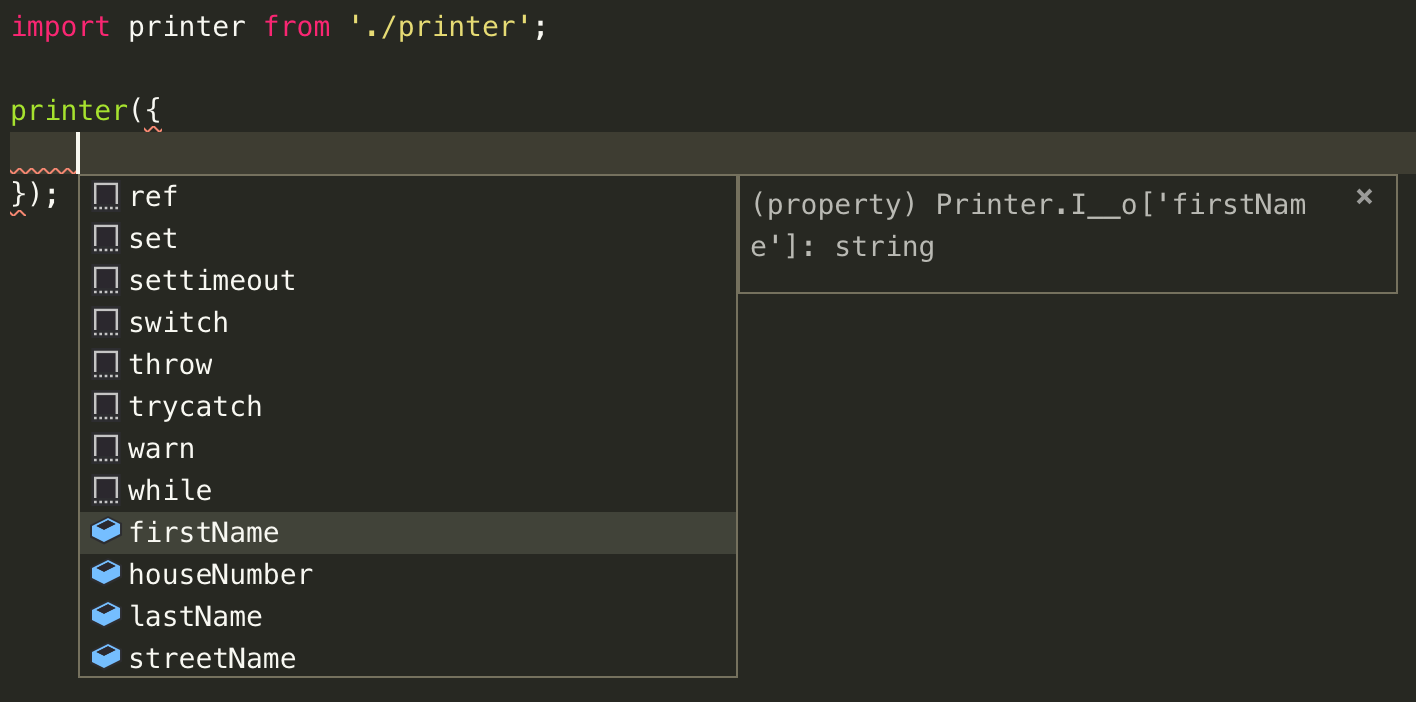
\includegraphics[width=1\textwidth]{figures/approach/typescript-declaration-files-generation-method/examples/example-with-interfaces/code-intelligence-vscode.png}}

	\caption[Declaration file generation example]{\textbf{Declaration file generation example} - Declaration file for the \mintinline{bash}{calculator} module is generated using the \mintinline{bash}{module-class.d.ts} template. Declaration file can be used within a TypeScript project: code intelligence features work as expected and the generated JavaScript file after compilation can be correctly executed.}
	\label{fig:run-time-information-gathering-get-field}
\end{figure}